%!TEX program = xelatex
\documentclass{beamer}

\usepackage{algorithm}
\usepackage{algorithmic}
\usepackage{graphicx}
\usepackage{booktabs}
\usepackage[T1]{fontenc}

\beamertemplatetransparentcovereddynamicmedium

\usepackage{listings}
\usepackage{color}

\usetheme{Darmstadt}
\usecolortheme{whale}

\definecolor{mygreen}{rgb}{0,0.6,0}
\definecolor{mygray}{rgb}{0.5,0.5,0.5}
\definecolor{mymauve}{rgb}{0.58,0,0.82}

\lstset{
  backgroundcolor=\color{white},   % choose the background color; you must add \usepackage{color} or \usepackage{xcolor}
  basicstyle=\footnotesize,        % the size of the fonts that are used for the code
  breakatwhitespace=false,         % sets if automatic breaks should only happen at whitespace
  breaklines=true,                 % sets automatic line breaking
  captionpos=b,                    % sets the caption-position to bottom
  commentstyle=\color{mygreen},    % comment style
  escapeinside={\%*}{*)},          % if you want to add LaTeX within your code
  extendedchars=true,              % lets you use non-ASCII characters; for 8-bits encodings only, does not work with UTF-8
  frame=single,                    % adds a frame around the code
  keepspaces=true,                 % keeps spaces in text, useful for keeping indentation of code (possibly needs columns=flexible)
  keywordstyle=\bfseries\color{blue},% keyword style
  language=C++,                    % the language of the code
  morekeywords={constexpr,decltype},% if you want to add more keywords to the set
  numbers=left,                    % where to put the line-numbers; possible values are (none, left, right)
  numbersep=5pt,                   % how far the line-numbers are from the code
  numberstyle=\tiny\color{mygray}, % the style that is used for the line-numbers
  rulecolor=\color{black},         % if not set, the frame-color may be changed on line-breaks within not-black text (e.g. comments (green here))
  showspaces=false,                % show spaces everywhere adding particular underscores; it overrides 'showstringspaces'
  showstringspaces=false,          % underline spaces within strings only
  showtabs=false,                  % show tabs within strings adding particular underscores
  stepnumber=1,                    % the step between two line-numbers. If it's 1, each line will be numbered
  stringstyle=\color{mymauve},     % string literal style
  tabsize=4,                       % sets default tabsize to 2 spaces
  %title=\lstname                  % show the filename of files included with \lstinputlisting; also try caption instead of title
  %caption=\lstname
}

\begin{document}
	\begin{frame}[containsverbatim]
		\title{Magi Language Compiler}
		\author{Zhijian LIU}
		\institute{Shanghai Jiao Tong University}
		\date{\today}
		\titlepage
	\end{frame}
	
	\begin{frame}
		\frametitle{The Gift of the Magi}
		\textbf{The Gift of the Magi} is a short story, written by O. Henry, about a young married couple and how they deal with the challenge of buying secret Christmas gifts for each other with very little money. As a sentimental story with a moral lesson about gift-giving, it has been a popular one for adaptation, especially for presentation at Christmas time. The plot and its "twist ending" are well-known, and the ending is generally considered an example of comic irony.
	\end{frame}
	
	\begin{frame}
		\frametitle{Project Overview}
		\begin{itemize}
			\item Time period: from \textbf{Mar 22} to \textbf{May 13}
			\item Git commits: \textbf{172} commits
			\item Java code length: \textbf{13485} lines
		\end{itemize}
	\end{frame}
	
	\begin{frame}
		\frametitle{Highlights}
		\begin{itemize}
			\item Use a well-organized framework with good extensibility
			\item<0-0> Feed back a user-friendly compilation error message
			\item<0-0> Support most features of \textbf{OOP} including member function, private modifier, class inheritance, member initialization and constructor function
			\item<0-0> Achieve an outstanding compilation quality
			\item<0-0> Implement the \textbf{SSA} form and do some optimizations on it including the useless code elimination and dominator-based value numbering technique
			\item<0-0> Do not use any peephole and data-oriented optimizations
			\item<0-0> Use the \textbf{global} register allocation and improve the algorithm
			\item<0-0> Make good use of the version control system
		\end{itemize}
	\end{frame}
	
	\begin{frame}
		\frametitle{Highlights}
		\begin{itemize}
			\item Use a well-organized framework with good extensibility
			\item Feed back a user-friendly compilation error message
			\item<0-0> Support most features of \textbf{OOP} including member function, private modifier, class inheritance, member initialization and constructor function
			\item<0-0> Achieve an outstanding compilation quality
			\item<0-0> Implement the \textbf{SSA} form and do some optimizations on it including the useless code elimination and dominator-based value numbering technique
			\item<0-0> Do not use any peephole and data-oriented optimizations
			\item<0-0> Use the \textbf{global} register allocation and improve the algorithm
			\item<0-0> Make good use of the version control system
		\end{itemize}
	\end{frame}

	\begin{frame}
		\frametitle{Demonstration: Compilation Error Message}
		\begin{itemize}
			\item \texttt{1:31: the function "angry" cannot have two parameters named "haha"!}
			\item \texttt{2:4: "haha" is not a symbol name!}
			\item \texttt{6:10: the number of parameters in the function-call expression is wrong!}
			\item \texttt{7:12: two int/string-type expressions are expected in the addition expression!}
		\end{itemize}
	\end{frame}

	\begin{frame}
		\frametitle{Highlights}
		\begin{itemize}
			\item Use a well-organized framework with good extensibility
			\item Feed back a user-friendly compilation error message
			\item Support most features of \textbf{OOP} including member function, private modifier, class inheritance, member initialization and constructor function
			\item<0-0> Achieve an outstanding compilation quality
			\item<0-0> Implement the \textbf{SSA} form and do some optimizations on it including the useless code elimination and dominator-based value numbering technique
			\item<0-0> Do not use any peephole and data-oriented optimizations
			\item<0-0> Use the \textbf{global} register allocation and improve the algorithm
			\item<0-0> Make good use of the version control system
		\end{itemize}
	\end{frame}

	\begin{frame}
		\frametitle{Demonstration: Object Oriented Programming}
		\begin{figure}[!htp]
			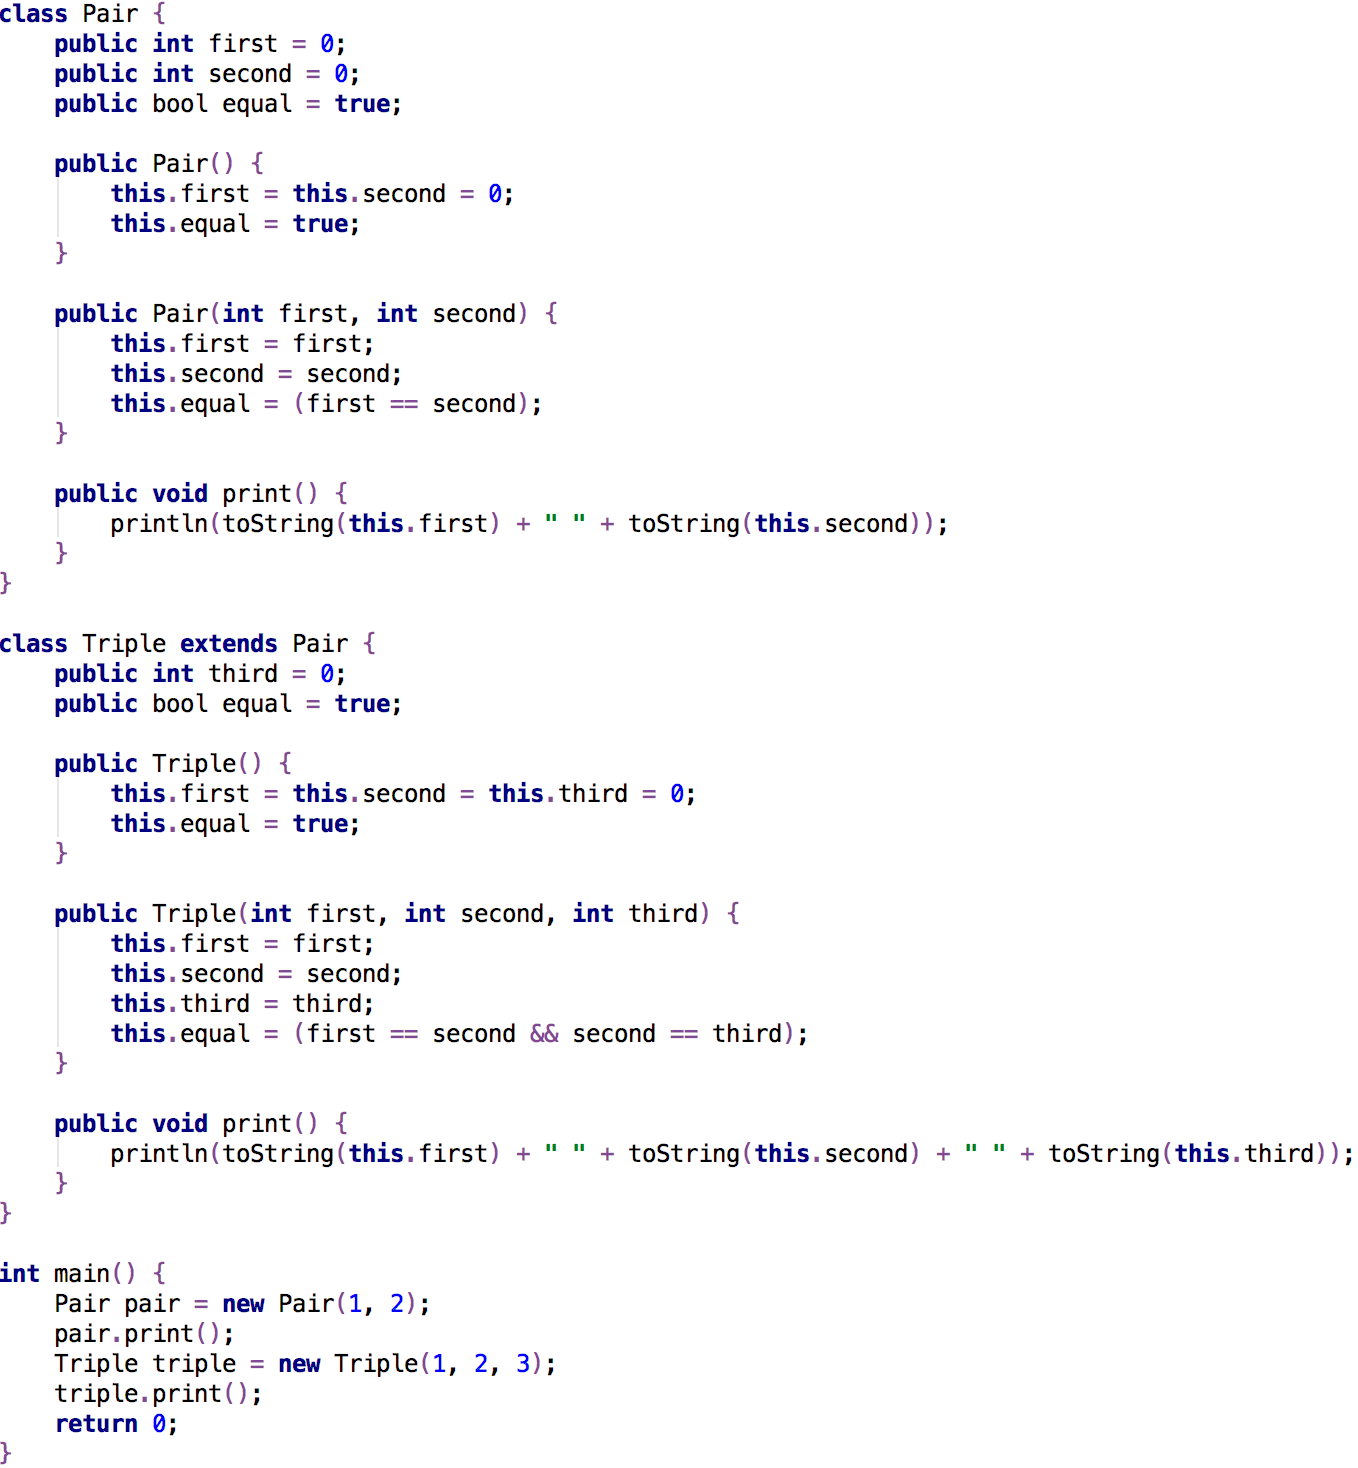
\includegraphics[height=7cm]{image/object-oriented-programming}
		\end{figure}
	\end{frame}
	
	\begin{frame}
		\frametitle{Highlights}
		\begin{itemize}
			\item Use a well-organized framework with good extensibility
			\item Feed back a user-friendly compilation error message
			\item Support most features of \textbf{OOP} including member function, private modifier, class inheritance, member initialization and constructor function
			\item Achieve an outstanding compilation quality
			\item<0-0> Implement the \textbf{SSA} form and do some optimizations on it including the useless code elimination and dominator-based value numbering technique
			\item<0-0> Do not use any peephole and data-oriented optimizations
			\item<0-0> Use the \textbf{global} register allocation and improve the algorithm
			\item<0-0> Make good use of the version control system
		\end{itemize}
	\end{frame}

	\begin{frame}
		\frametitle{Demonstration: Normalized Benchmark Result}
		\begin{figure}[!htp]
			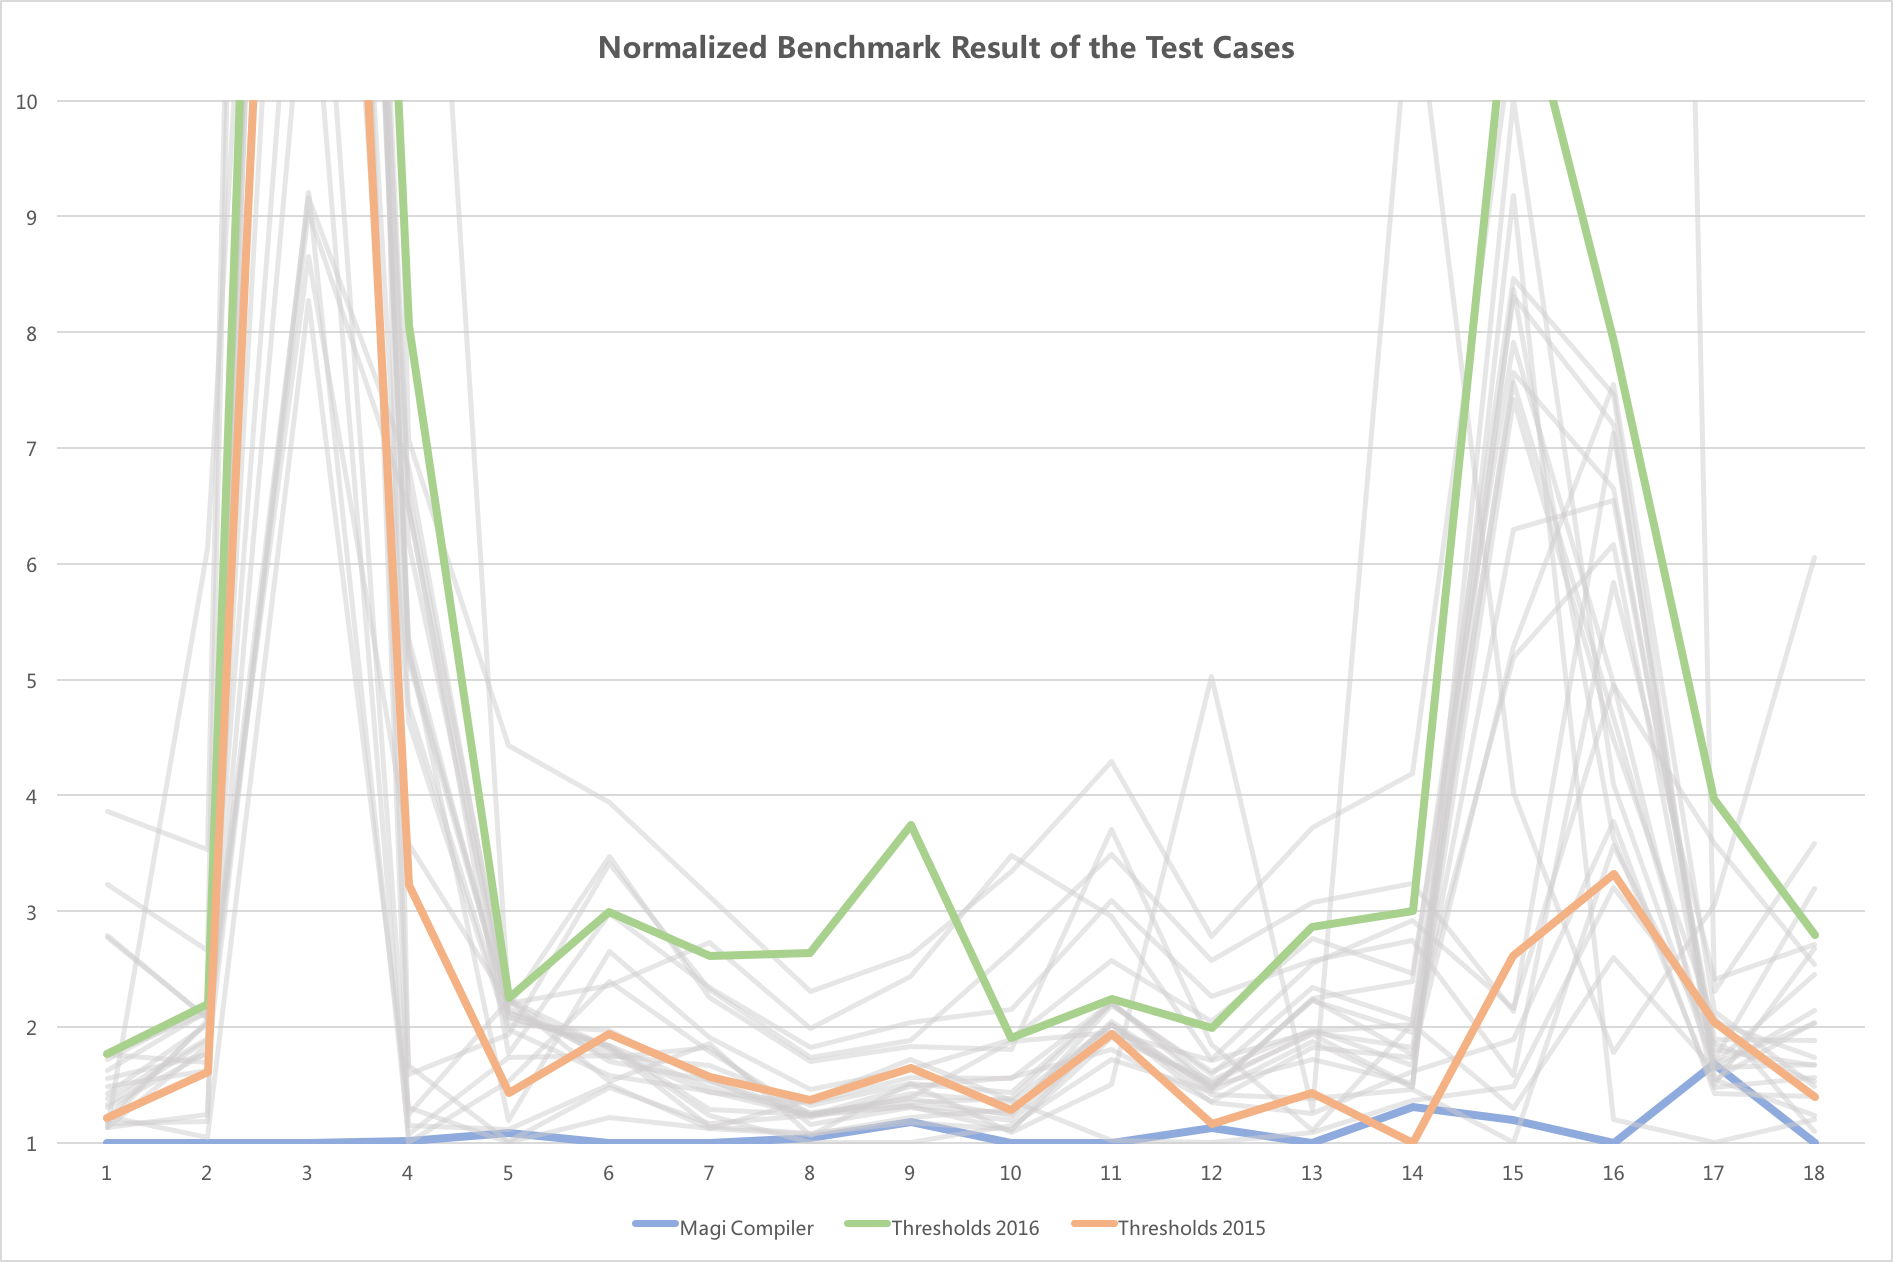
\includegraphics[height=6.5cm]{image/benchmark/thresholds}
		\end{figure}
	\end{frame}

	\begin{frame}
		\frametitle{Highlights}
		\begin{itemize}
			\item Use a well-organized framework with good extensibility
			\item Feed back a user-friendly compilation error message
			\item Support most features of \textbf{OOP} including member function, private modifier, class inheritance, member initialization and constructor function
			\item Achieve an outstanding compilation quality
			\item Implement the \textbf{SSA} form and do some optimizations on it including the useless code elimination and dominator-based value numbering technique
			\item<0-0> Do not use any peephole and data-oriented optimizations
			\item<0-0> Use the \textbf{global} register allocation and improve the algorithm
			\item<0-0> Make good use of the version control system
		\end{itemize}
	\end{frame}

	\begin{frame}
		\frametitle{Demonstration: Single Static Assignment}
		\begin{figure}[!htp]
			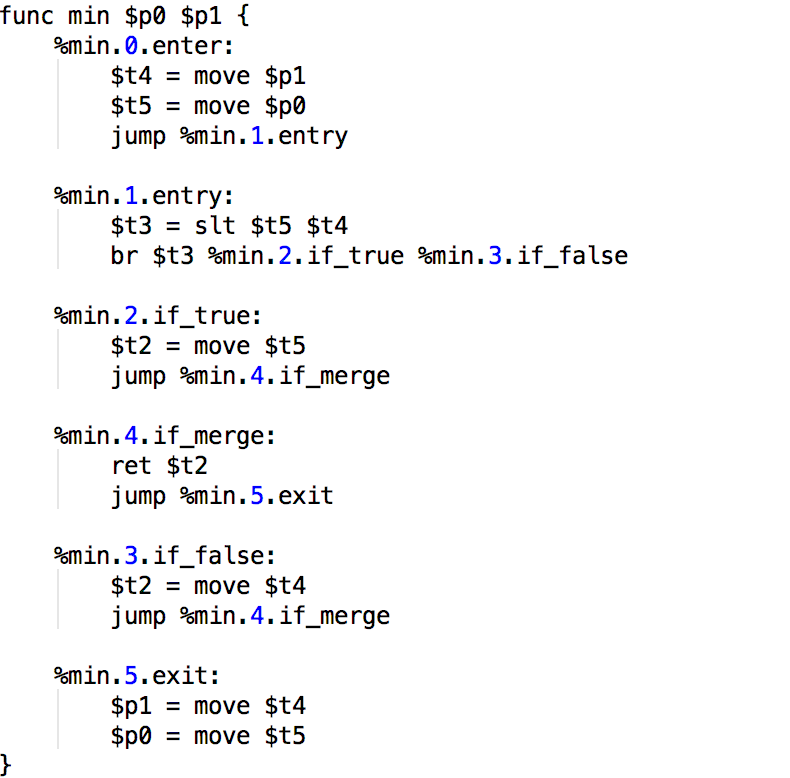
\includegraphics[height=6.5cm]{image/single-static-assignment/before-single-static-assignment}
		\end{figure}
	\end{frame}
	
	\begin{frame}
		\frametitle{Demonstration: Single Static Assignment}
		\begin{figure}[!htp]
			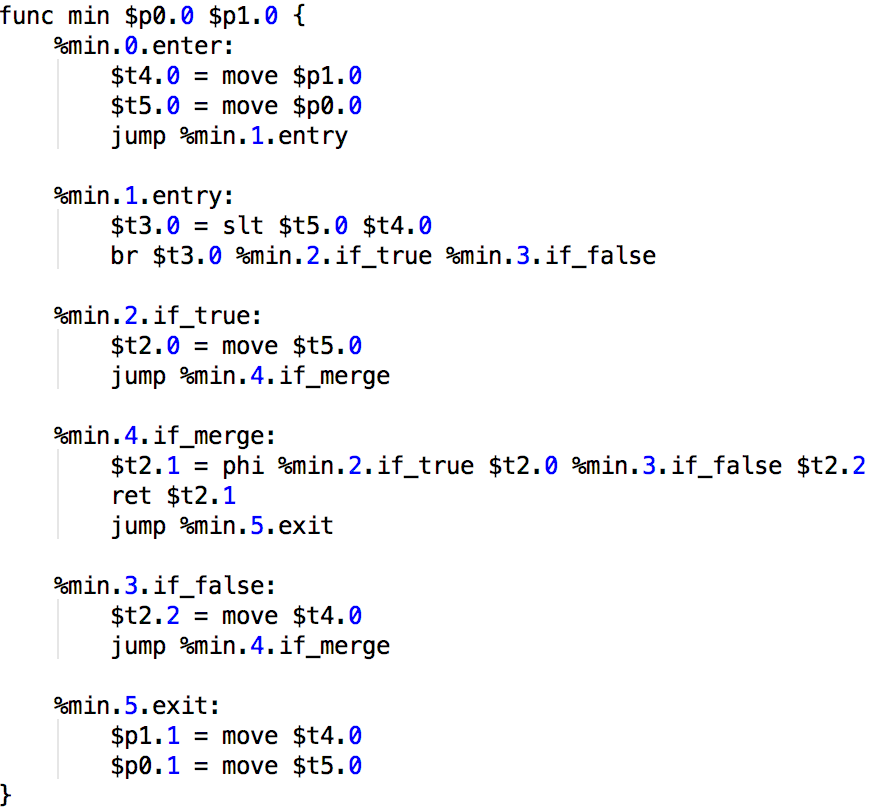
\includegraphics[height=6.5cm]{image/single-static-assignment/after-single-static-assignment}
		\end{figure}
	\end{frame}

	\begin{frame}
		\frametitle{Demonstration: Normalized Benchmark Result}
		\begin{figure}[!htp]
			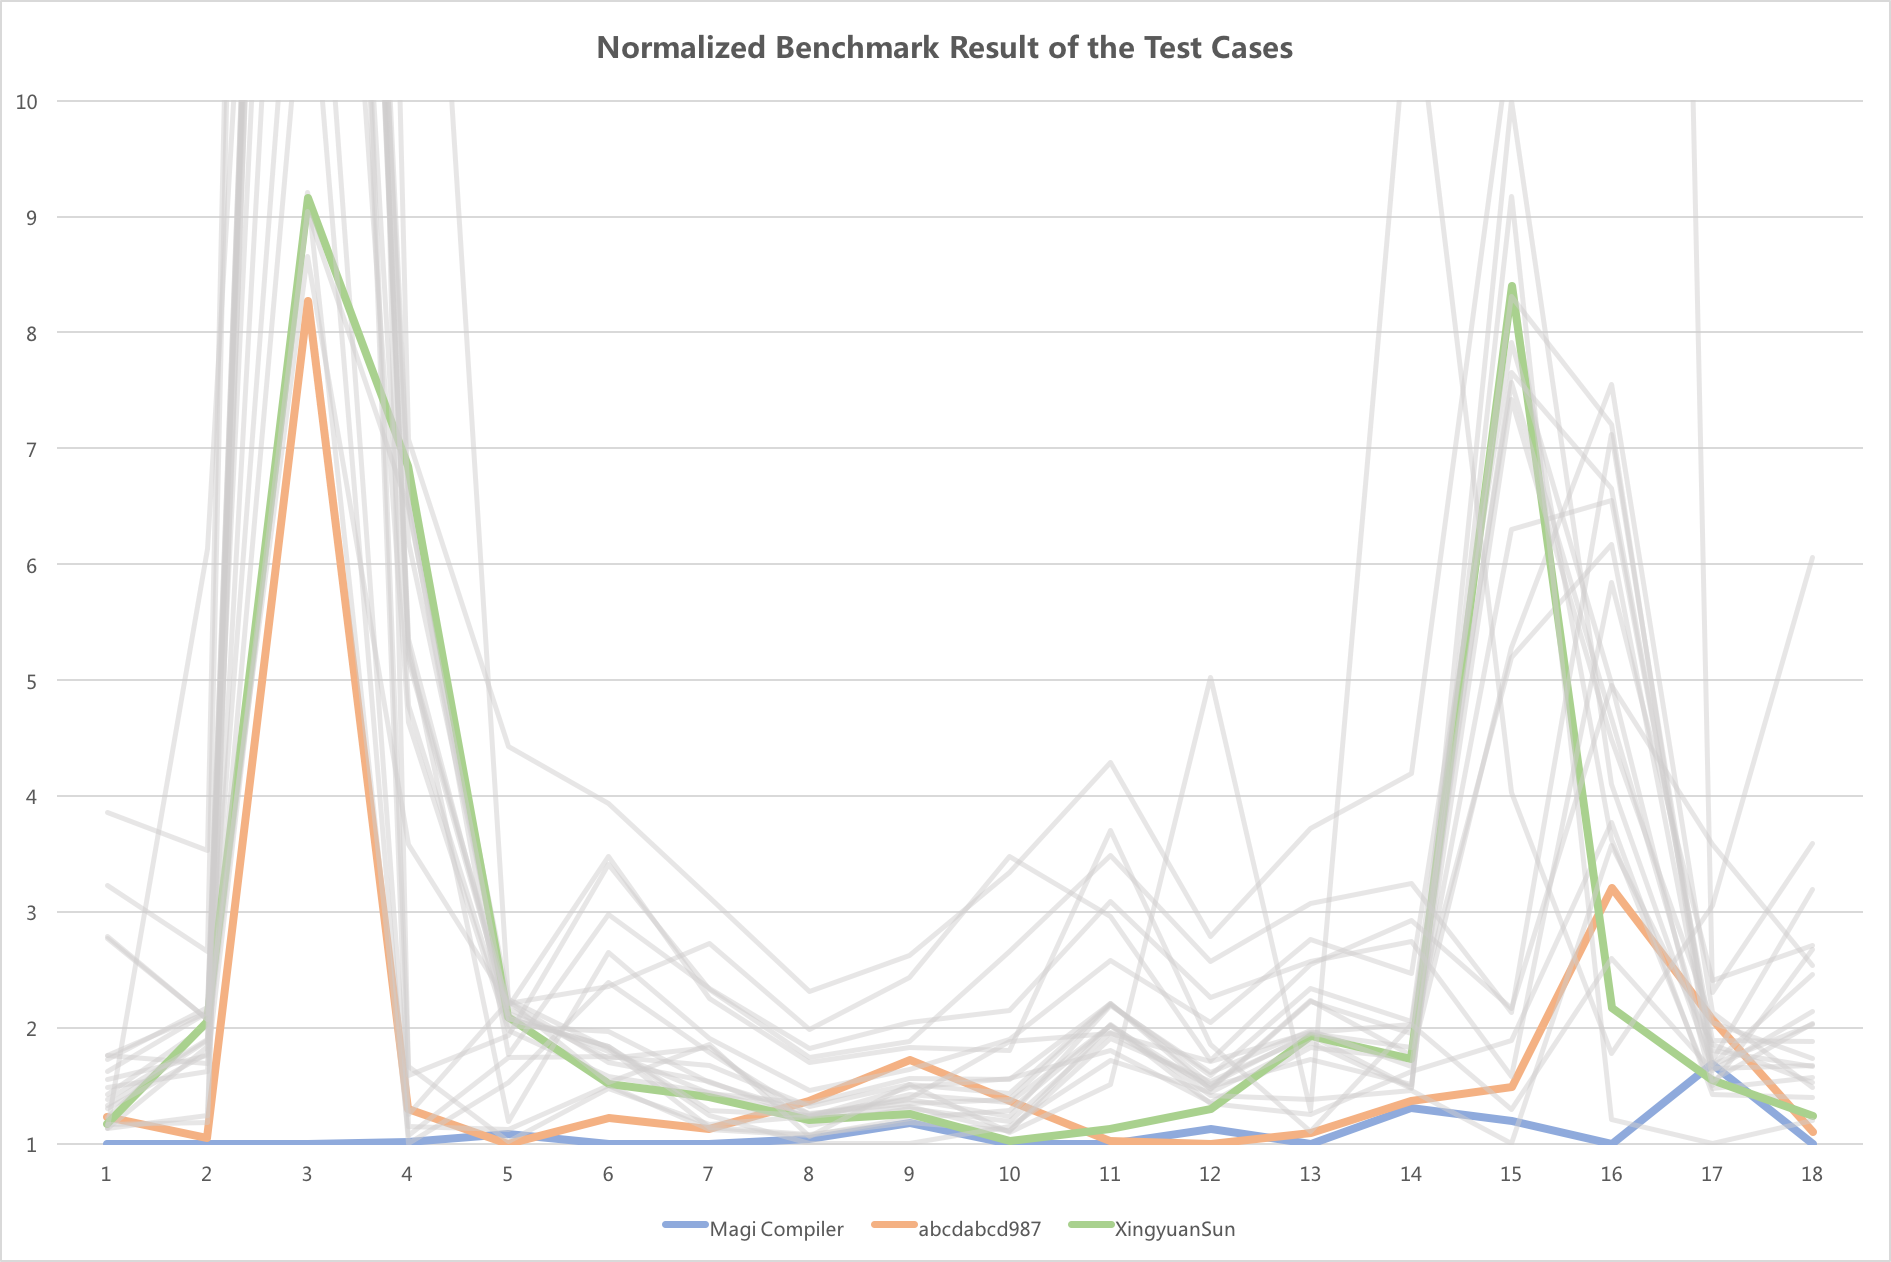
\includegraphics[height=6.5cm]{image/benchmark/single-static-assignment}
		\end{figure}
	\end{frame}

	\begin{frame}
		\frametitle{Highlights}
		\begin{itemize}
			\item Use a well-organized framework with good extensibility
			\item Feed back a user-friendly compilation error message
			\item Support most features of \textbf{OOP} including member function, private modifier, class inheritance, member initialization and constructor function
			\item Achieve an outstanding compilation quality
			\item Implement the \textbf{SSA} form and do some optimizations on it including the useless code elimination and dominator-based value numbering technique
			\item Do not use any peephole and data-oriented optimizations
			\item<0-0> Use the \textbf{global} register allocation and improve the algorithm
			\item<0-0> Make good use of the version control system
		\end{itemize}
	\end{frame}

	\begin{frame}
		\frametitle{Demonstration: Normalized Benchmark Result}
		\begin{figure}[!htp]
			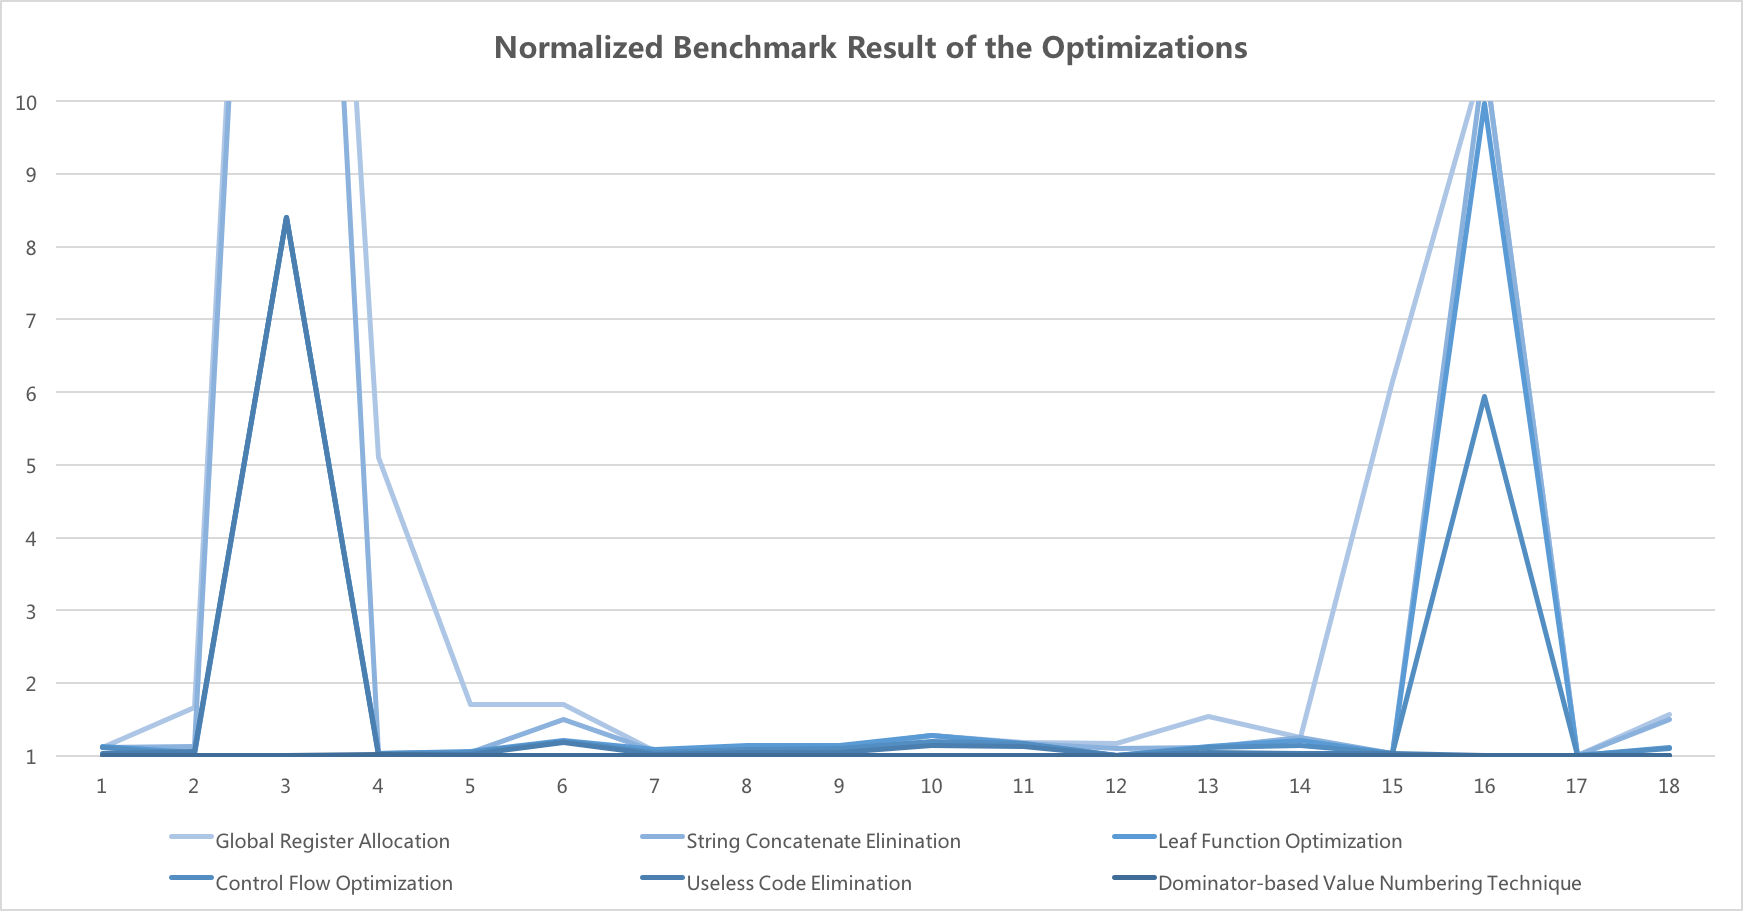
\includegraphics[height=5.5cm]{image/benchmark/optimization}
		\end{figure}
	\end{frame}

	\begin{frame}
		\frametitle{Highlights}
		\begin{itemize}
			\item Use a well-organized framework with good extensibility
			\item Feed back a user-friendly compilation error message
			\item Support most features of \textbf{OOP} including member function, private modifier, class inheritance, member initialization and constructor function
			\item Achieve an outstanding compilation quality
			\item Implement the \textbf{SSA} form and do some optimizations on it including the useless code elimination and dominator-based value numbering technique
			\item Do not use any peephole and data-oriented optimizations
			\item Use the \textbf{global} register allocation and improve the algorithm
			\item<0-0> Make good use of the version control system
		\end{itemize}
	\end{frame}

	\begin{frame}
		\frametitle{Demonstration: Normalized Benchmark Result}
		\begin{figure}[!htp]
			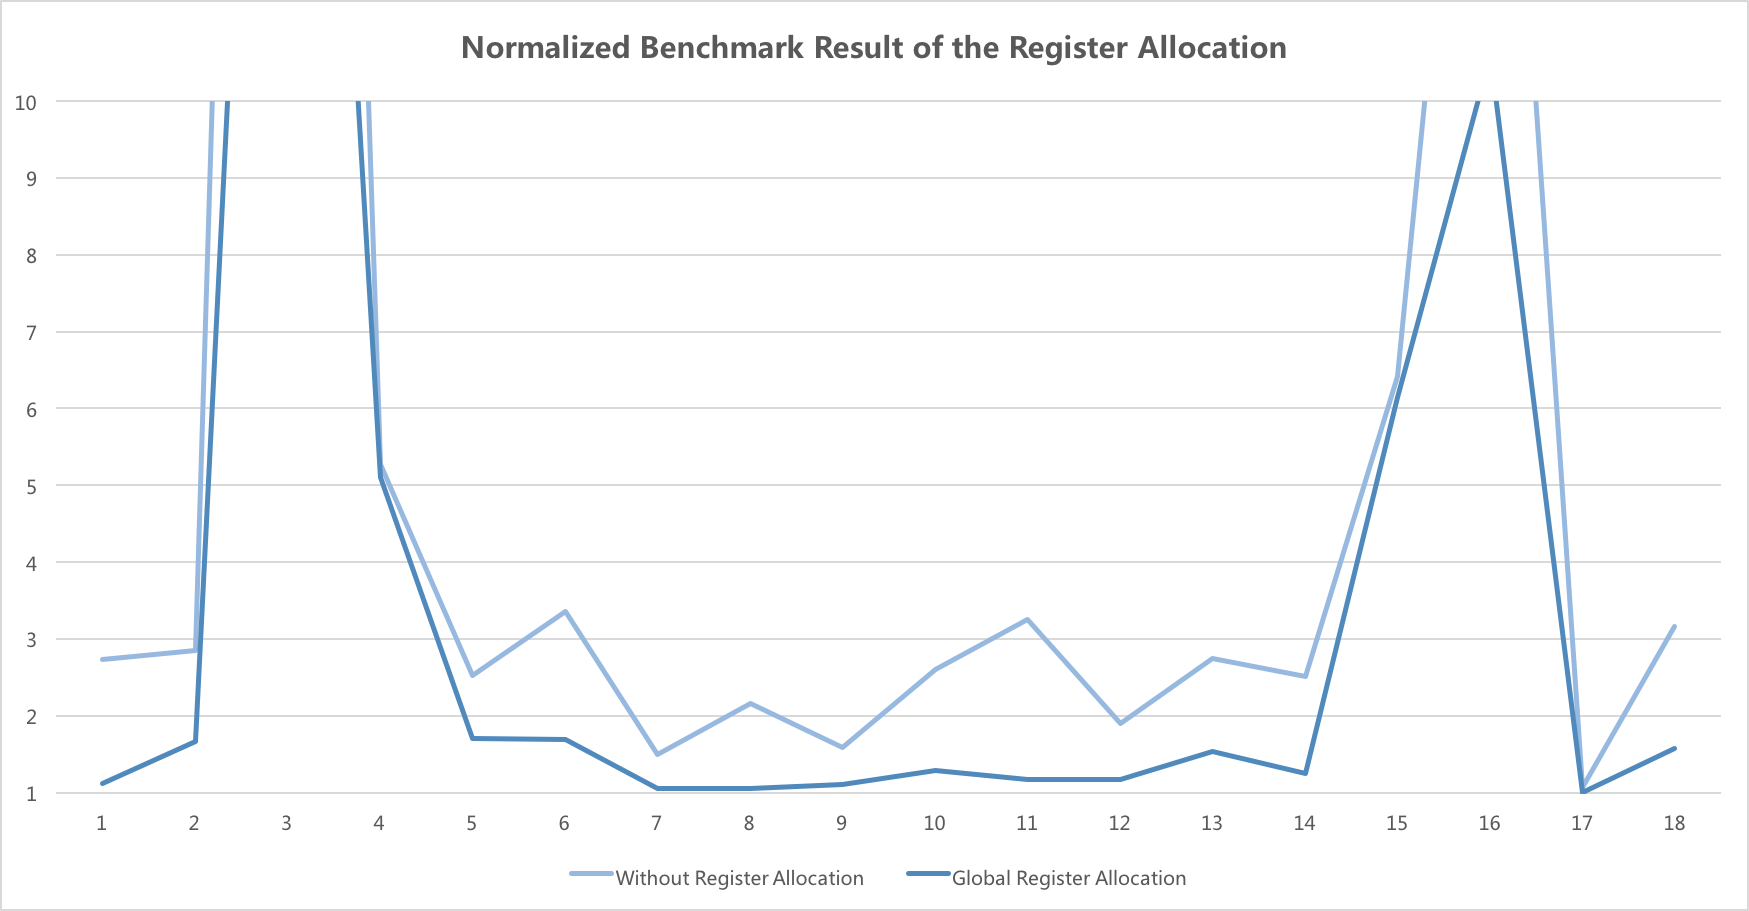
\includegraphics[height=5.5cm]{image/benchmark/register-allocation}
		\end{figure}
	\end{frame}

	\begin{frame}
		\frametitle{Highlights}
		\begin{itemize}
			\item Use a well-organized framework with good extensibility
			\item Feed back a user-friendly compilation error message
			\item Support most features of \textbf{OOP} including member function, private modifier, class inheritance, member initialization and constructor function
			\item Achieve an outstanding compilation quality
			\item Implement the \textbf{SSA} form and do some optimizations on it including the useless code elimination and dominator-based value numbering technique
			\item Do not use any peephole and data-oriented optimizations
			\item Use the \textbf{global} register allocation and improve the algorithm
			\item Make good use of the version control system
		\end{itemize}
	\end{frame}

	\begin{frame}
		\frametitle{Front End}
		\begin{enumerate}
			\item Use \textbf{AN}other \textbf{T}ool for \textbf{L}anguage \textbf{R}ecognition to generate the lexer and parser
			\item Convert the \textbf{C}oncrete \textbf{S}yntax \textbf{T}ree to the \textbf{A}bstract \textbf{S}yntax \textbf{T}ree by the listener mode of \textbf{ANTLR}
		\end{enumerate}
	\end{frame}

	\begin{frame}
		\frametitle{Abstract Syntax Tree Framework}
		\begin{figure}[!htp]
			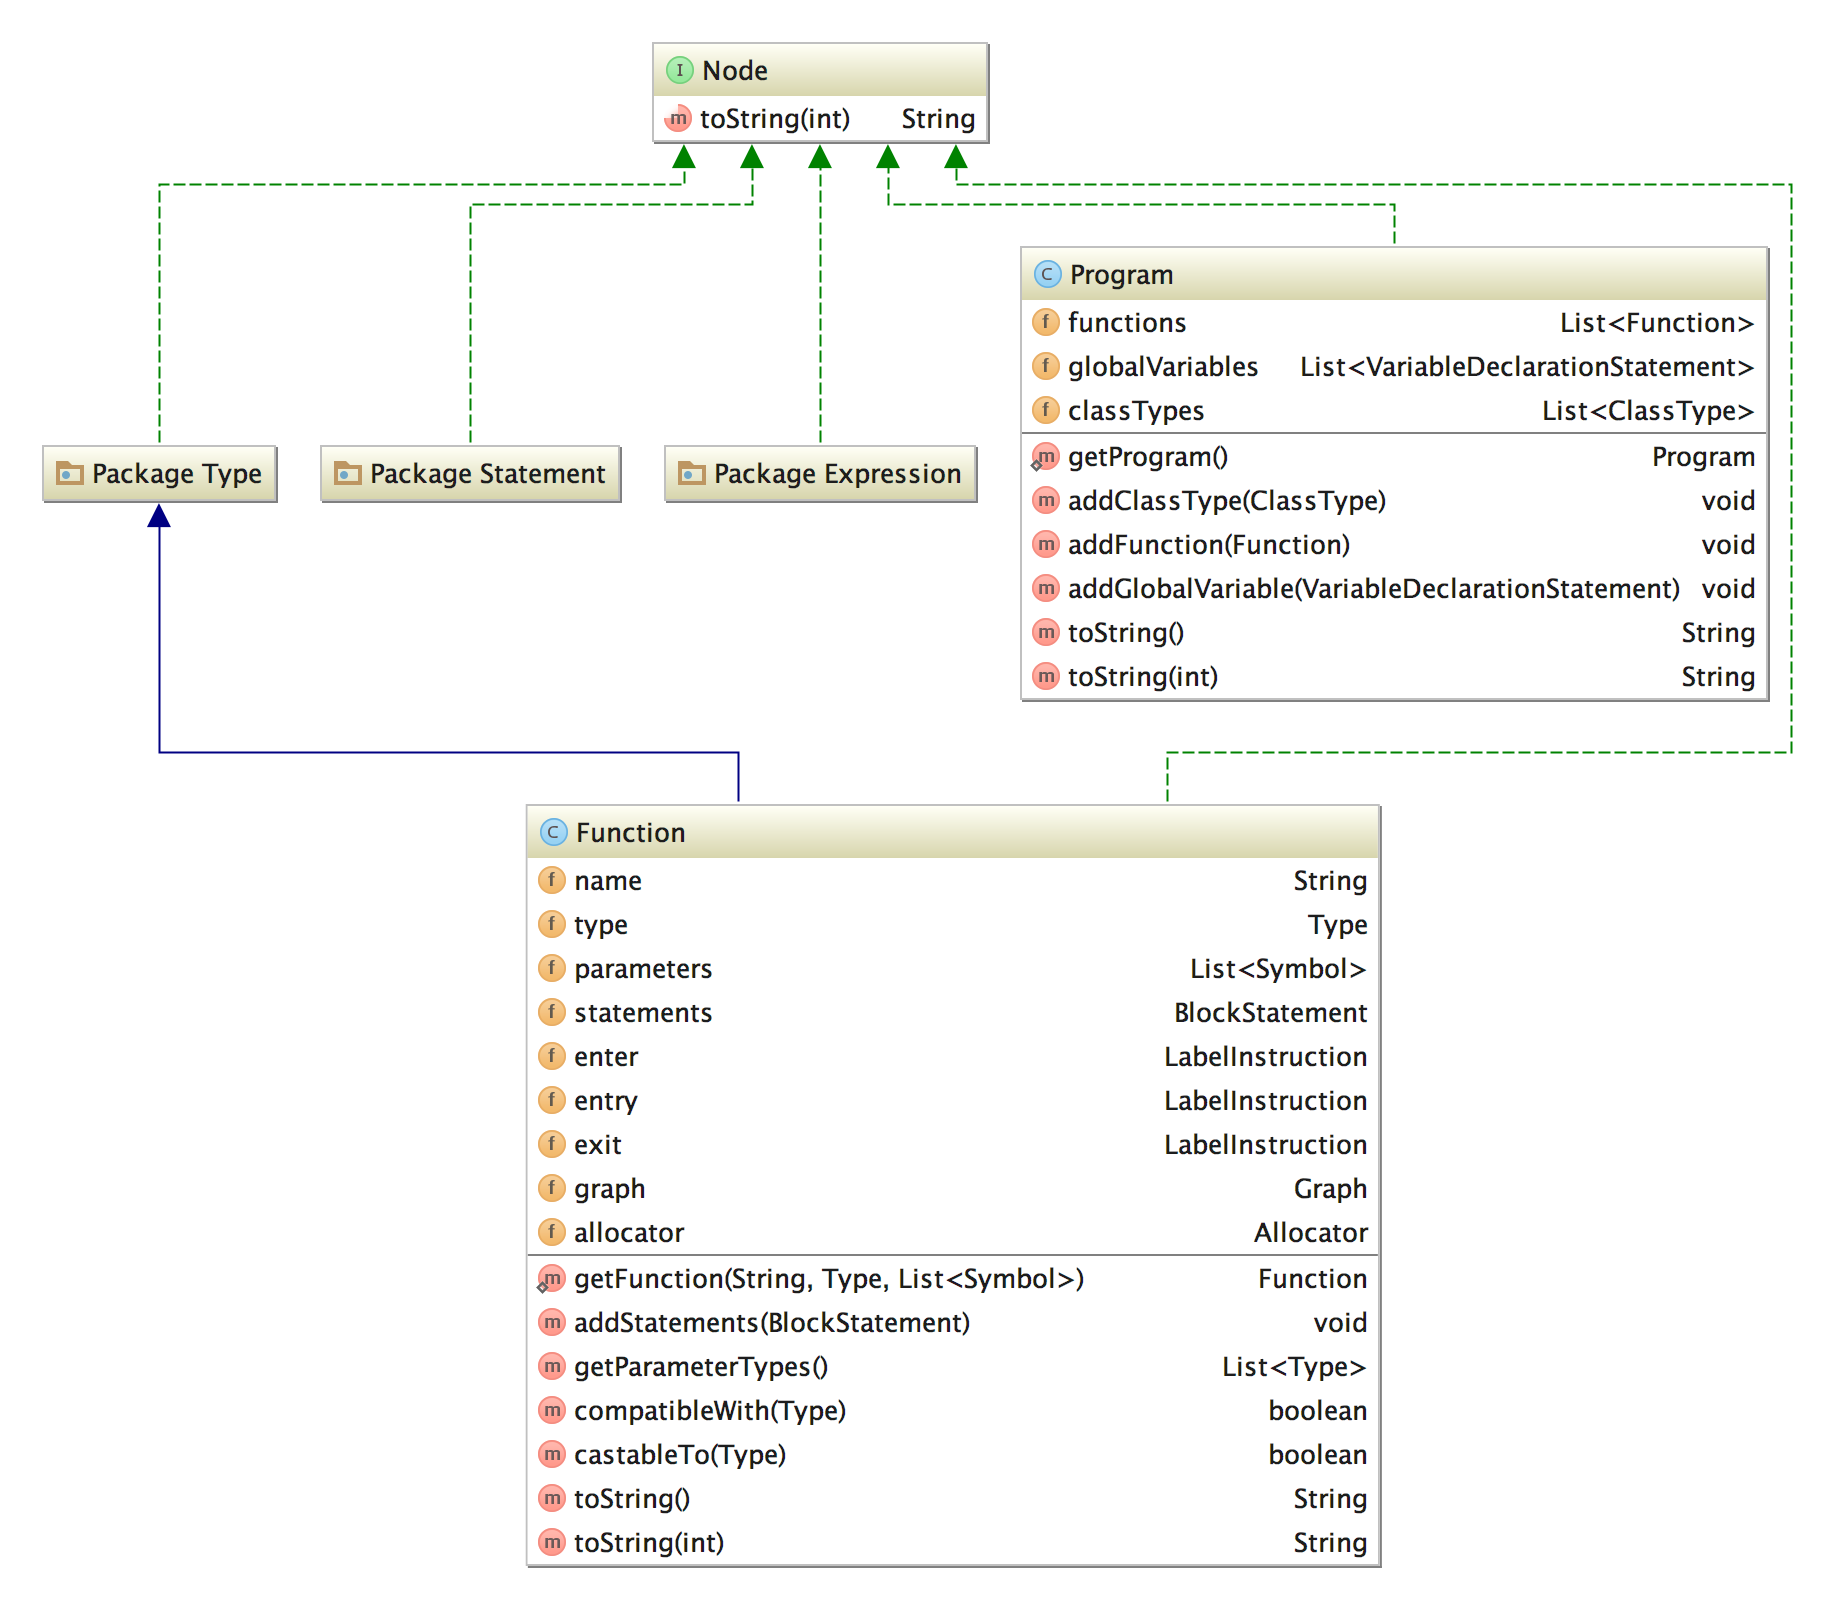
\includegraphics[height=6.5cm]{image/abstract-syntax-tree}
		\end{figure}
	\end{frame}
	
	\begin{frame}
		\frametitle{Back End}
		\begin{enumerate}
			\item Convert the \textbf{A}bstract \textbf{S}yntax \textbf{T}ree to the linear \textbf{I}ntermediate \textbf{R}epresentation
			\item Build the \textbf{C}ontrol \textbf{F}low \textbf{G}raph by scanning the linear \textbf{I}ntermediate \textbf{R}epresentation
		\end{enumerate}
	\end{frame}

	\begin{frame}
		\frametitle{Intermediate Representation Framework}
		\begin{figure}[!htp]
			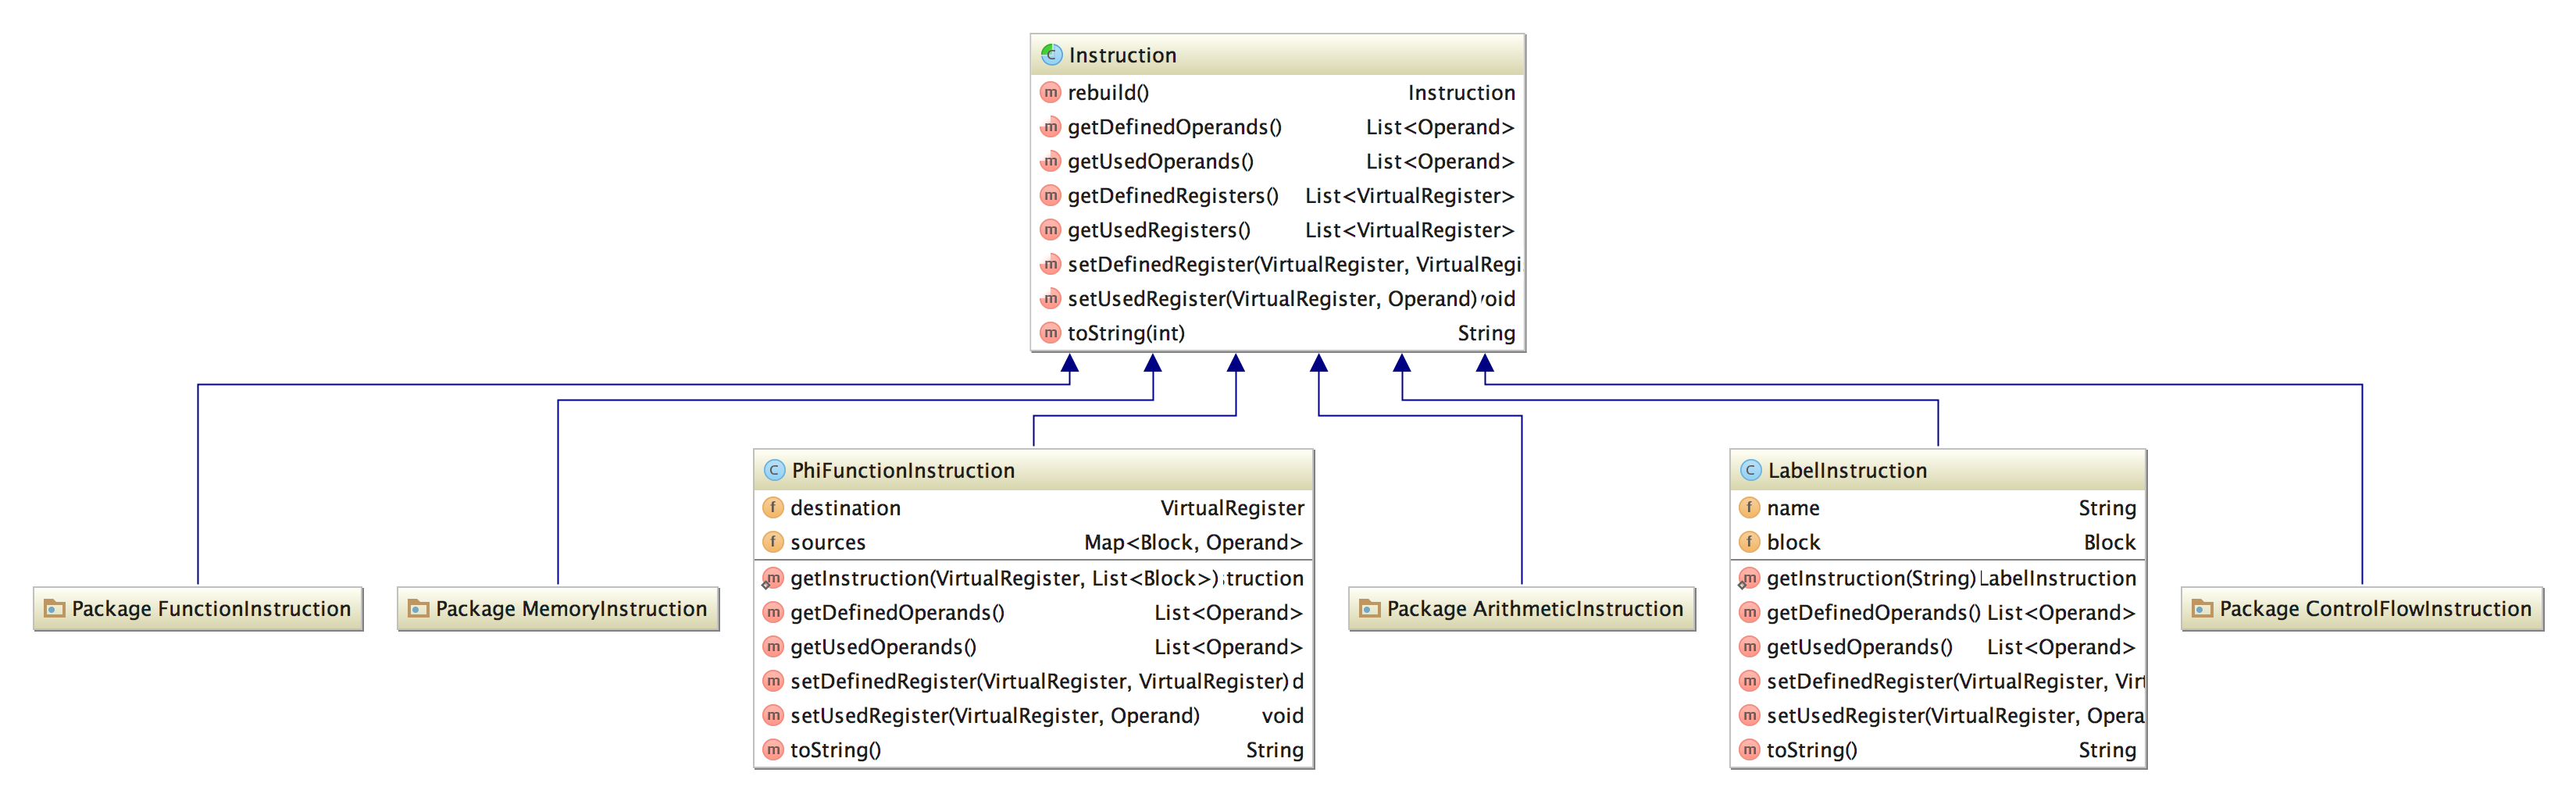
\includegraphics[height=3cm]{image/intermediate-representation}
		\end{figure}
	\end{frame}
	
	\begin{frame}
		\frametitle{Single Static Assignment}
		\begin{figure}[!htp]
			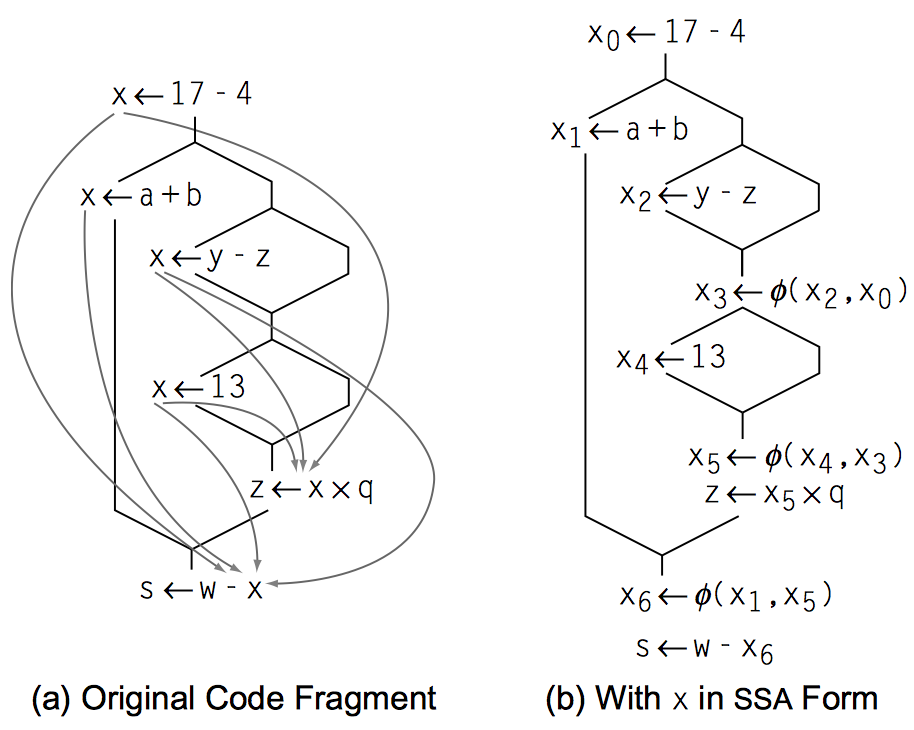
\includegraphics[height=5.5cm]{image/single-static-assignment/single-static-assignment}
		\end{figure}
	\end{frame}

	\begin{frame}
		\frametitle{Single Static Assignment}
		\begin{enumerate}
			\item Compute the immediate dominator and the dominance frontier
			\item Insert $\phi$-functions
			\item Rename the variables and the temporaries
			\item Do some optimizations based on SSA form
			\item Translate out of SSA form
		\end{enumerate}
	\end{frame}
	
	\begin{frame}
		\frametitle{Single Static Assignment: Analyze the Dominance}
		\begin{block}{Definition}
			In a flow graph with entry node $s$, node $u$ \textbf{dominates} node $v$ iff $u$ lies on every path from $s$ to $v$
		\end{block}
		\pause
		\begin{alertblock}{Data flow equation}
			\[
				\text{dom}_v = \{v\} \cup \left(\bigcap_{p \in pred_v}{dom_p} \right)
			\]
		\end{alertblock}
	\end{frame}

	\begin{frame}
		\frametitle{Single Static Assignment: Analyze the Dominance}
		\begin{block}{Definitions}
			\begin{itemize}
				\item A node $u$ \textbf{strictly dominates} a node $v$ if $u$ dominates $v$ and $u$ does not equal $v$.
				\item The \textbf{immediate dominator} of a node $u$ is the unique node that strictly dominates $u$ but does not strictly dominate any other node that strictly dominates $u$.
				\item The \textbf{dominance frontier} of a node $u$ is the set of all nodes $v$ such that $u$ dominates an immediate \textbf{predecessor} of $v$, but $u$ does not strictly dominate $v$. It is the set of nodes where $u$'s dominance stops.
			\end{itemize}
		\end{block}
	\end{frame}

	\begin{frame}
		\frametitle{Single Static Assignment: Immediate Dominator}
		\begin{figure}[!htp]
			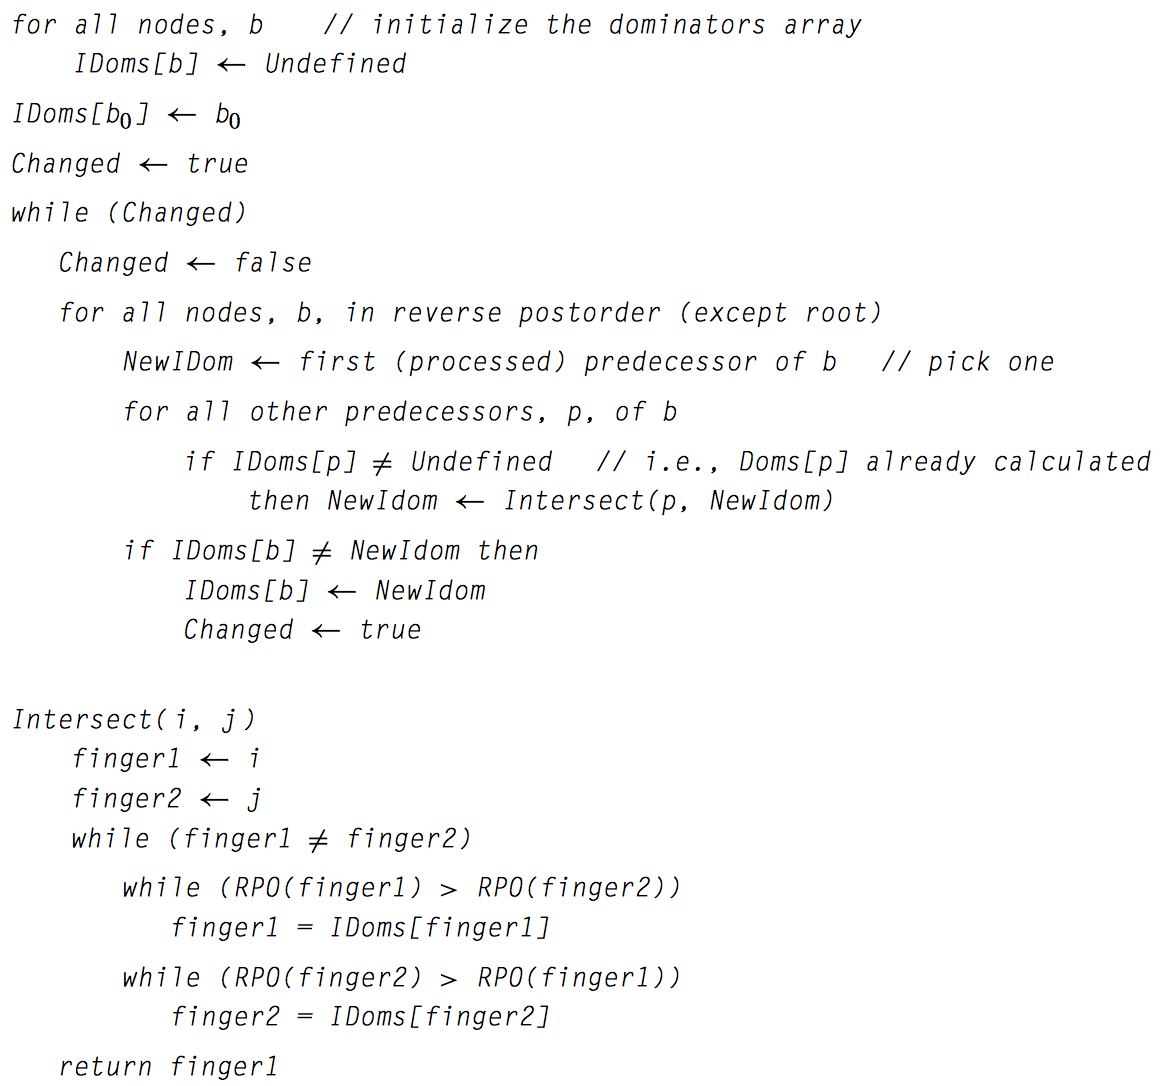
\includegraphics[height=6.5cm]{image/single-static-assignment/compute-the-dominators}
		\end{figure}
	\end{frame}

	\begin{frame}
		\frametitle{Single Static Assignment: Insert $\phi$-functions}
		\begin{figure}[!htp]
			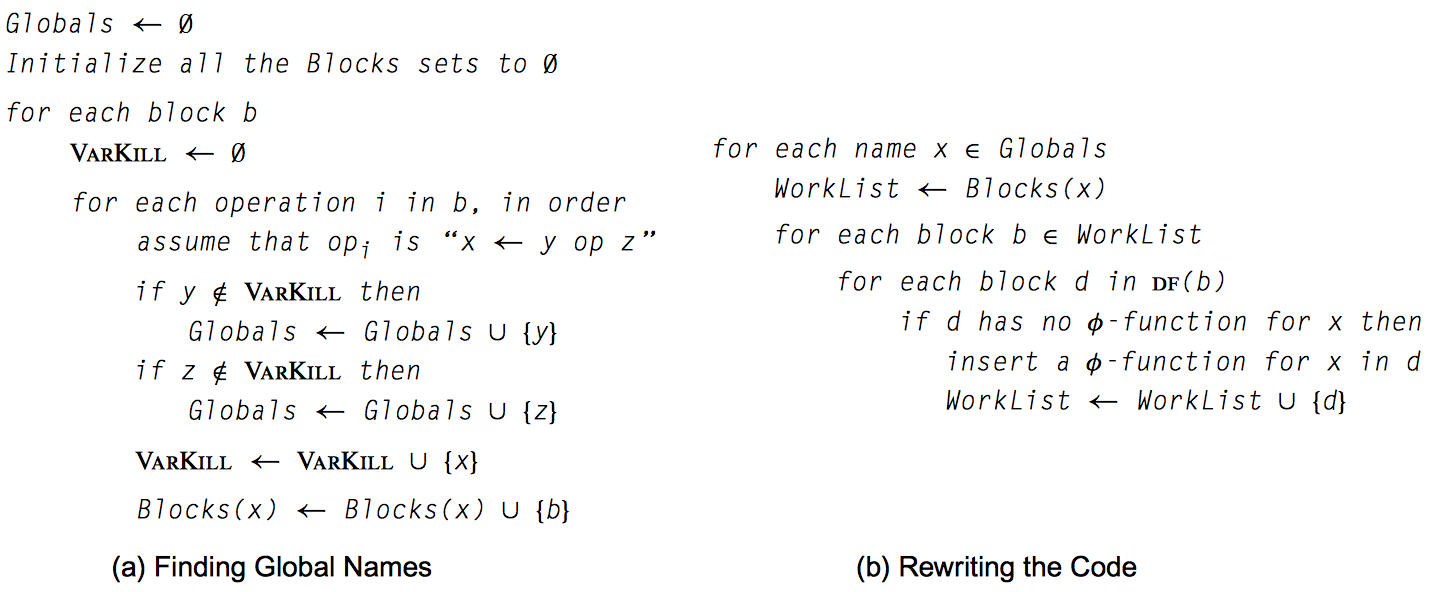
\includegraphics[height=4.5cm]{image/single-static-assignment/insert-phi-functions}
		\end{figure}
	\end{frame}

	\begin{frame}
		\frametitle{Single Static Assignment: Rename the Variables}
		\begin{figure}[!htp]
			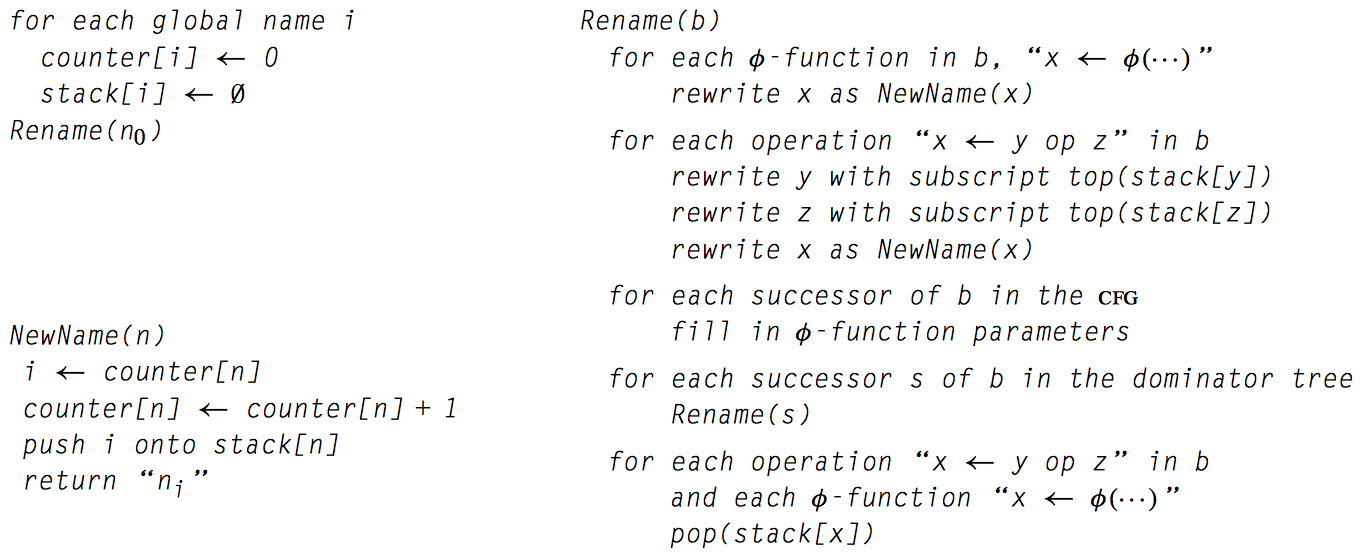
\includegraphics[height=4.5cm]{image/single-static-assignment/rename-the-variables}
		\end{figure}
	\end{frame}
	
	\begin{frame}
		\frametitle{Optimizations}
		\begin{block}{Regular optimizations}
			\begin{enumerate}
				\item Leaf function optimization
				\item Control flow optimization
			\end{enumerate}
		\end{block}
		\begin{alertblock}{Optimizations based on SSA form}
			\begin{enumerate}
			\item Useless code elimination
			\item Dominator-based value numbering technique
			\end{enumerate}
		\end{alertblock}
	\end{frame}
	
	\begin{frame}
		\frametitle{Optimization: Control Flow Optimization}
		\begin{figure}[!htp]
			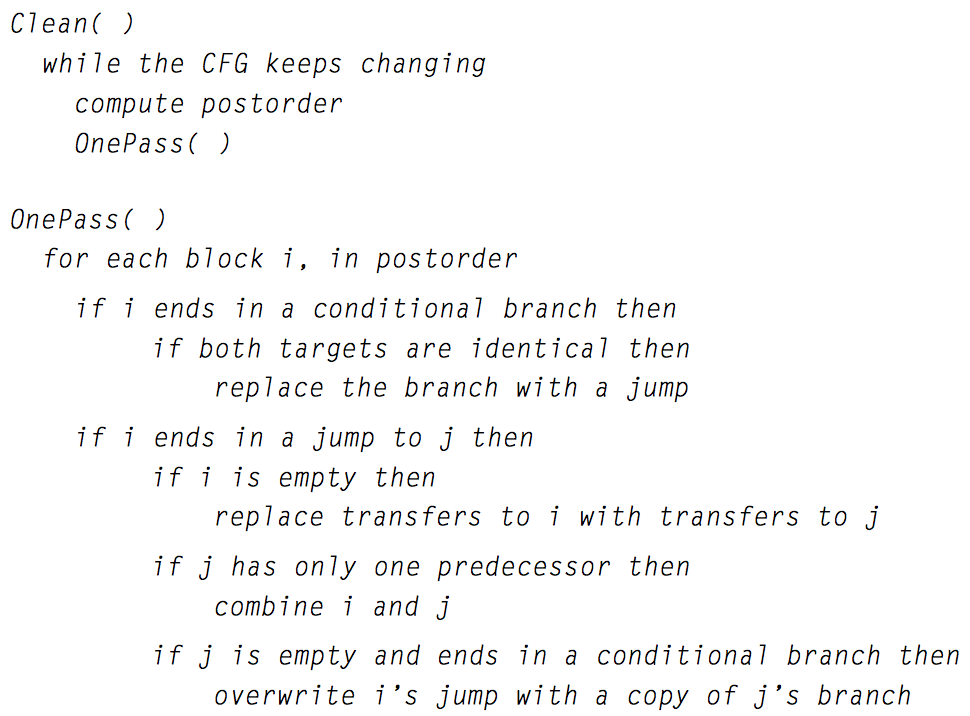
\includegraphics[height=5.5cm]{image/optimization/control-flow-optimization}
		\end{figure}
	\end{frame}

	\begin{frame}
		\frametitle{Optimization: Useless Code Elimination}
		\begin{figure}[!htp]
			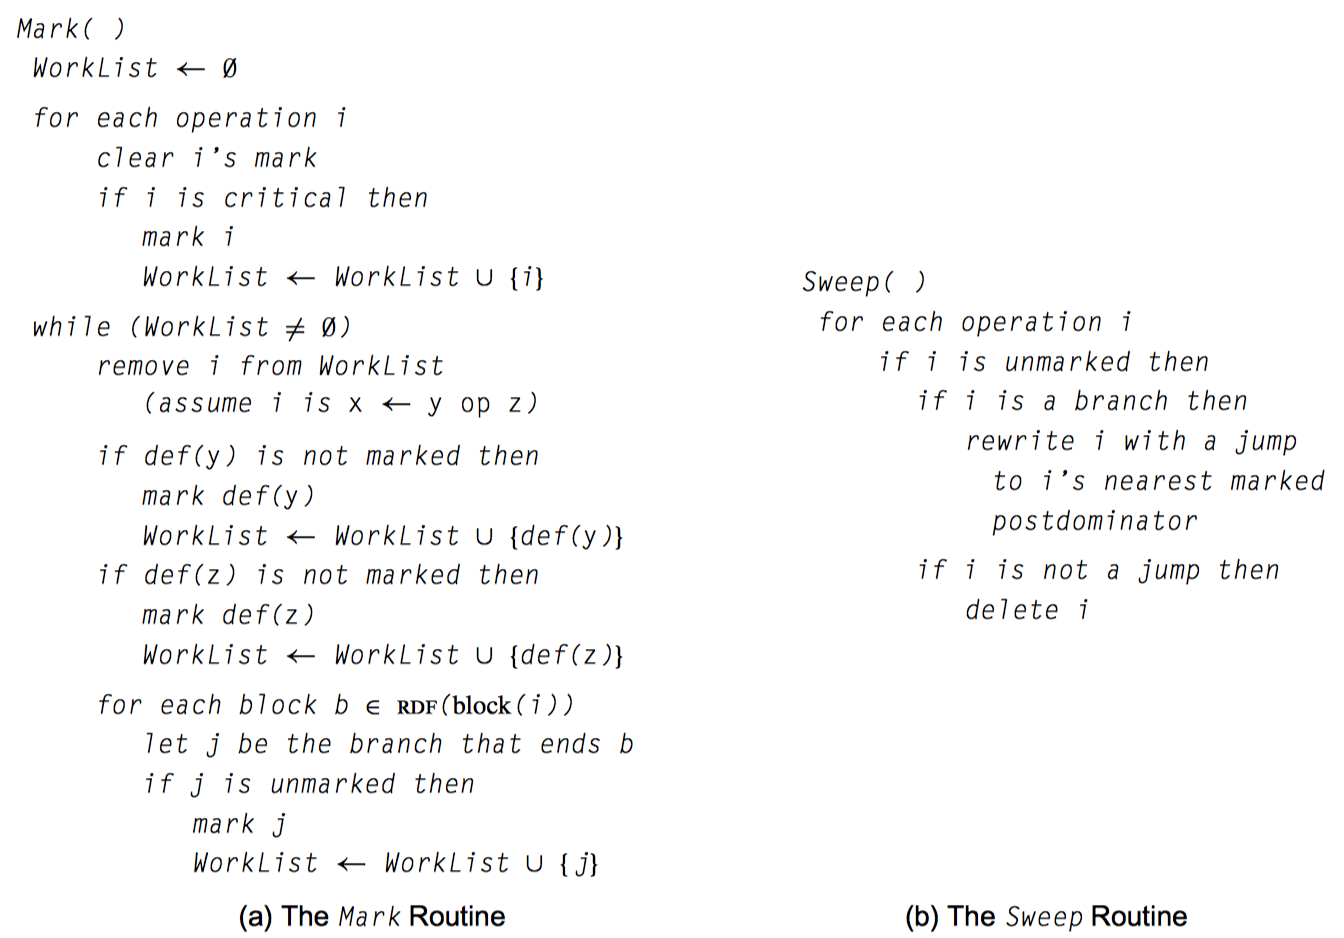
\includegraphics[height=6.5cm]{image/optimization/useless-code-elimination}
		\end{figure}
	\end{frame}

	\begin{frame}
		\frametitle{Optimization: Dominator-based Value Numbering}
		\begin{figure}[!htp]
			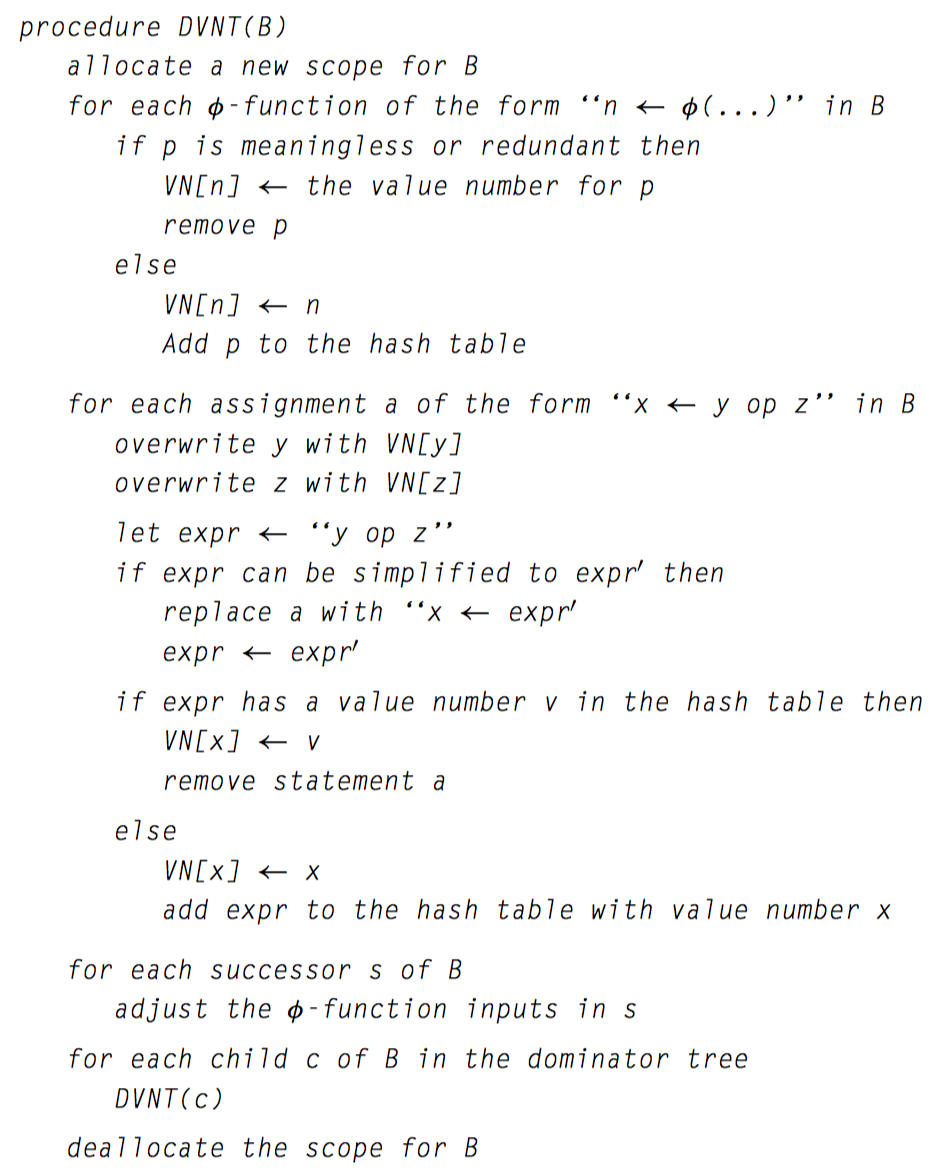
\includegraphics[height=6.5cm]{image/optimization/dominator-based-value-numbering-technique}
		\end{figure}
	\end{frame}

	\begin{frame}
		\frametitle{Global Register Allocation}
		\begin{enumerate}
			\item Analyze the liveliness
			\item Build the interference graph
			\item Use the bottom-up coloring
		\end{enumerate}
	\end{frame}
	
	\begin{frame}
		\frametitle{Global Register Allocation: Liveliness Analysis}
		\begin{block}{Definitions}
			\begin{itemize}
				\item $v$ \textbf{live} at $e$ iff there is a path $p$ from $e$ to $i$ such that
				\begin{itemize}
					\item instruction $i$ uses $v$
					\item no instructions defining $v$ on the path $p$
				\end{itemize}
				\item $v$ \textbf{live-in} at $i$ iff $v$ \textbf{live} at $e$, where $e \in in\text{-}edge_i$
				\item $v$ \textbf{live-out} at $i$ iff $v$ \textbf{live} at $e$, where $e \in out\text{-}edge_i$ 
			\end{itemize}
		\end{block}
		\pause
		\begin{alertblock}{Data flow equation}
			\[
			\begin{aligned}
				live\text{-}in_i &= use_i \cup \left(live\text{-}out_i \setminus def_i\right)\\
				live\text{-}out_i &= \bigcup_{s \in succ_i}{live\text{-}in_s}
			\end{aligned}
			\]
		\end{alertblock}
	\end{frame}

	\begin{frame}
		\frametitle{Global Register Allocation: Liveliness Analysis}
		\begin{enumerate}
			\item Calculate the $def$ and $use$ for each basic block
			\item Do the liveliness analysis on each basic block by using \textbf{the fix-point algorithm}
			\item Calculate the liveliness information for each instruction in each basic block by \textbf{the one-pass backward calculation}
		\end{enumerate}
	\end{frame}

	\begin{frame}
		\frametitle{Global Register Allocation: Interference Graph}
		\begin{itemize}
			\item For a \textbf{move} instruction $i$,
				\\ \quad add \textbf{forbidden} edges between $def_i$ and $\text{live-out}_i \setminus use_i$
				\\ \quad add \textbf{recommend} edges between $def_i$ and $use_i$
			\item For a \textbf{non-move} instruction $i$,
				\\ \quad add \textbf{forbidden} edges between $def_i$ and $\text{live-out}_i$
		\end{itemize}
	\end{frame}

	\begin{frame}
		\frametitle{Global Register Allocation: Bottom-up Coloring}
		\setcounter{algorithm}{0}
		\begin{algorithm}[H]
			\caption{Computing the coloring order for $G = (V, E)$}
			\begin{algorithmic}[1]
				\STATE initialize $stack$ to empty
				\WHILE{$V$ is not empty}
					\IF{$\exists v \in V$ with $deg_v < k$}
						\STATE $candidate \leftarrow v$
					\ELSE
						\STATE $candidate \leftarrow v$ \textbf{picked} from $V$
					\ENDIF
					\STATE remove $candidate$ and its edges in the graph $G$
					\STATE push $candidate$ onto $stack$
				\ENDWHILE
			\end{algorithmic}
		\end{algorithm}
	\end{frame}

	\begin{frame}
		\frametitle{Global Register Allocation: Bottom-up Coloring}
		\setcounter{algorithm}{1}
		\begin{algorithm}[H]
			\caption{Coloring bottom-up for $G = (V, E)$}
			\begin{algorithmic}[1]
				\WHILE{$stack$ is not empty}
					\STATE $v \leftarrow pop\left(stack\right)$
					\STATE insert $v$ and its edges into the graph $G$
					\STATE \textbf{color} $v$
				\ENDWHILE
			\end{algorithmic}
		\end{algorithm}
	\end{frame}
	
	\begin{frame}
		\frametitle{Other work}
		\begin{itemize}
			\item<1-> Give some of my classmates advice on the framework and optimization
			\item<2-> Provide some \textbf{IR} test data for my classmates
			\item<3-> Provide a unit test file for my classmates
			\item<4-> Help some of my classmates with debugging
		\end{itemize}
	\end{frame}
	
	\begin{frame}
		\frametitle{Summary}
		\begin{itemize}
			\item I am ashamed to do only a little bit of the work
			\item Thank all of you, my \textbf{TA}s and my classmates
		\end{itemize}
	\end{frame}
\end{document}
